\scanpage{43}
% archive sheet number: 42
\diagram{\begin{tikzcd}[ampersand replacement=\&]
\mathscr H^1(X;A)\arrow[d,dash]\&\mathrm{Ext}^1(A,\mathrm{Pic})\\
\text{pt singulier}\&
\end{tikzcd}}
\[
\boxed{\mathscr H^1(X,G)\simeq\mathrm{Hom}(D(G),\underline{\mathrm{Pic}}_{X})}
\]
\figure{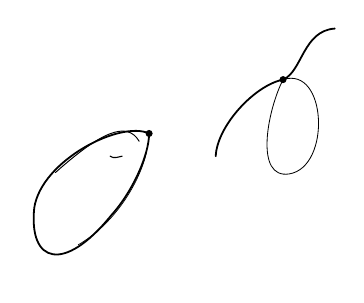
\begin{tikzpicture}[x=.009cm,y=-.009cm,line cap=round,line join=round]
\draw[line width=.65pt] (165,152) .. controls (125,133) and (13,190) .. (3,257) .. controls (-5,335) and (45,350) .. (112,267) .. controls (141,235) and (165,183) .. (165,152);
\draw[line width=.35pt] (33,207) .. controls (98,149) and (134,134) .. (151,163);
\draw[line width=.25pt] (65,309) .. controls (116,280) and (151,222) .. (161,180);
\draw (110,184) .. controls (115,188) and (122,185) .. (127,184);
\fill (165,152) circle (5);
\draw[line width=.65pt] (259,184) .. controls (261,141) and (314,84) .. (354,76) .. controls (381,65) and (382,7) .. (427,4);
\draw[line width=.3pt] (354,76) .. controls (332,119) and (313,217) .. (363,209) .. controls (422,199) and (416,56) .. (354,76);
\fill (354,76) circle (5);
\end{tikzpicture}}
\[
\mathscr H^{i}(X,D(G))\simeq\mathrm{Ext}^{i}(G,\underline{\mathrm{Pic}}_{X})
\]
\[
\mathrm{Ext}^{i}_{X}(f^{!}(G),G_{m\unsure{,|{}}})\simeq\mathrm{Ext}^{i}_{Y}(G,f_{!}(G_{m}))
\]
\diagram{\begin{tikzcd}[ampersand replacement=\&]
X\arrow[d,"f"']\\Y
\end{tikzcd}}
\[
\boxed{\underline{\mathrm{Ext}}^{i}_{X}(f^{*}(G_{\cdot}),H^{\cdot})\simeq\underline{\mathrm{Ext}}^{i}_{Y}(G_{\cdot},f_{!}(H^{\cdot}))}
\]
\[
H=G_m
\]
\[
\underline{\mathrm{Ext}}^{i}_{X}(f^{*}(G),G_{m})\simeq\underline{\mathrm{Ext}}^{i}_{Y}(G,\overset{\text{\unsure{les supérieurs}}}{\tikz[baseline=(p.base)]\node[draw,ellipse,inner sep=2pt](p){$\underline{\mathrm{Pic}}^{\bullet}_{X/Y}$};})
\]
\[
\begin{aligned}
&\deleted{\unsure{f|R}}&&&&\Vert\\
&\deleted{\unsure{H^p(X,|H^i(X,}}&&\Vert
\end{aligned}
\]
\[
\boxed{G\text{ \uline{affine}, alors}\quad H^{i}(X,D(G))\Longleftarrow\deleted{\unsure{\mathscr H}}\mathrm{Ext}^{p}(G,\mathrm{Pic}^{(q)}_{X/Y})}
\]
\[
\begin{aligned}
\unsure{i|j}=0\qquad&H^0(X,D(G))=\deleted{\unsure{\mathrm{Hom}}}D(G)\\
i=1\qquad&H^1(X,D(G))=\deleted{\unsure{\mathrm{Ex}|\mathrm{Ext}}}\mathrm{Hom}(G,\mathrm{Pic}^{(1)})\\
i=2\qquad&\underline{H^2(X,D(\unsure{e|G}))\mathrel{\#}\mathrm{Ext}^1(G,\mathrm{Pic}^{(1)}_{X/Y})+\mathrm{Hom}(G,\underline{\mathrm{Pic}}^{\unsure{(2)}}_{X})}\\[-2pt]
&\hspace{4em}\text{!}
\end{aligned}
\]
$G$ abélien \quad Alors \quad \unsure{chg|sg}
\[
H^{i-1}(X,G')\Longleftarrow\mathrm{Ext}^{p}_{\unsure{\mathrm{gr}|Y}}(G,\mathrm{Pic}^{q}_{X/Y})
\]
\[
\begin{aligned}
i=0\qquad&0=0\\
i=1\qquad&H^{0}(X,G')=
\end{aligned}
\]
